\changecolours{ScoutBlue}
\section{O Teorema CAP}

% ------------------------------------------------------------------------------
\twocolframe[title={Origem Histórica e Formulação Formal do Teorema CAP},leftcol=7cm,rightcol=7cm]{%
  \alert{Eric Brewer (ACM PODC, 2000)}\par
  \itemseps[topsepi=2mm,itemsepi=3mm,labelsep=2mm,leftmargini=4mm]
  \begin{itemize}
    \item Proposto como uma conjectura pelo professor Eric Brewer (UC Berkeley) em 2000.
    \item Provado formalmente como teorema matemático em 2002 por \textbf{Seth Gilbert e Nancy Lynch} (MIT).
    \item Tornou-se o alicerce fundamental para a compreensão de todos os bancos de dados modernos.
  \end{itemize}
}{%
  \alert{O Enunciado Fundamental}\par
  \itemseps[topsepi=2mm,itemsepi=3mm,labelsep=2mm,leftmargini=4mm]
  \begin{itemize}
    \item Em qualquer sistema distribuído de dados sujeito a comunicação assíncrona por rede:
    \item \textbf{É matematicamente impossível garantir simultaneamente:}
      \begin{enumerate}
        \item Consistência (\textit{Consistency});
        \item Disponibilidade (\textit{Availability});
        \item Tolerância a Partições (\textit{Partition Tolerance}).
      \end{enumerate}
  \end{itemize}
}

% ------------------------------------------------------------------------------
\twocolframe[title={As 3 Propriedades do CAP em Detalhes Rigorosos},leftcol=7cm,rightcol=7cm]{%
  \alert{C: Consistência (Linearizabilidade)}\par
  \itemseps[topsepi=1.5mm,itemsepi=2.5mm,labelsep=2mm,leftmargini=4mm]
  \begin{itemize}
    \item Todo nó responde exatamente com o dado mais recente ou falha explicitamente.
    \item Comportamento idêntico a um sistema de máquina única centralizada.
  \end{itemize}
  \vspace{0.2cm}
  \alert{A: Disponibilidade (Availability)}\par
  \itemseps[topsepi=1.5mm,itemsepi=2.5mm,labelsep=2mm,leftmargini=4mm]
  \begin{itemize}
    \item Todo nó ativo e sem pane física \textbf{deve responder com sucesso} a qualquer requisição recebida (sem retornar erro 500/503 ou timeout).
  \end{itemize}
}{%
  \alert{P: Tolerância a Partições (Partition Tolerance)}\par
  \itemseps[topsepi=2mm,itemsepi=3mm,labelsep=2mm,leftmargini=4mm]
  \begin{itemize}
    \item Capacidade do sistema de continuar operando mesmo que mensagens entre os nós sejam perdidas, atrasadas ou descartadas.
    \item A partição ocorre fisicamente quando um cabo rompe ou roteador falha, dividindo o cluster em dois ou mais subconjuntos isolados (\textbf{Split-Brain}).
  \end{itemize}
}

% ------------------------------------------------------------------------------
\twocolframe[title={Desmistificando o CAP: Por que ``Escolha 2 de 3'' é Falso?},leftcol=7cm,rightcol=7cm]{%
  \alert{A Visão Antiga (O Triângulo Equivocado)}\par
  \itemseps[topsepi=2mm,itemsepi=3mm,labelsep=2mm,leftmargini=4mm]
  \begin{itemize}
    \item Muitos tutoriais de internet dizem erroneamente: \textit{``Basta escolher CA, CP ou AP''}.
    \item Afirmam que bancos como PostgreSQL ou MySQL seriam ``CA'' (Consistentes e Disponíveis).
    \item \textbf{O Erro Fatal:} Na internet e em redes de computadores, a Partição de Rede ($P$) \textbf{NUNCA é uma escolha}. Ela é um fato físico inegociável.
  \end{itemize}
}{%
  \alert{A Realidade (Brewer, 2012)}\par
  \itemseps[topsepi=2mm,itemsepi=3mm,labelsep=2mm,leftmargini=4mm]
  \begin{itemize}
    \item \textit{``CAP Twelve Years Later: How the Rules Have Changed''} (Eric Brewer, IEEE Computer 2012):
    \item Se a rede for 100\% perfeita e local (máquina única), você tem $C$ e $A$.
    \item \textbf{Mas quando ocorre uma partição de rede}, você é matematicamente forçado a escolher entre:
    \item \textbf{CP:} Preservar a consistência e sacrificar a disponibilidade; OU
    \item \textbf{AP:} Preservar a disponibilidade e sacrificar a consistência.
  \end{itemize}
}

% ------------------------------------------------------------------------------
\begin{frame}{O Teorema CAP na Prática: Mito vs. Realidade}
  \vspace{-0.3cm}
  \makebox[\linewidth][c]{%
    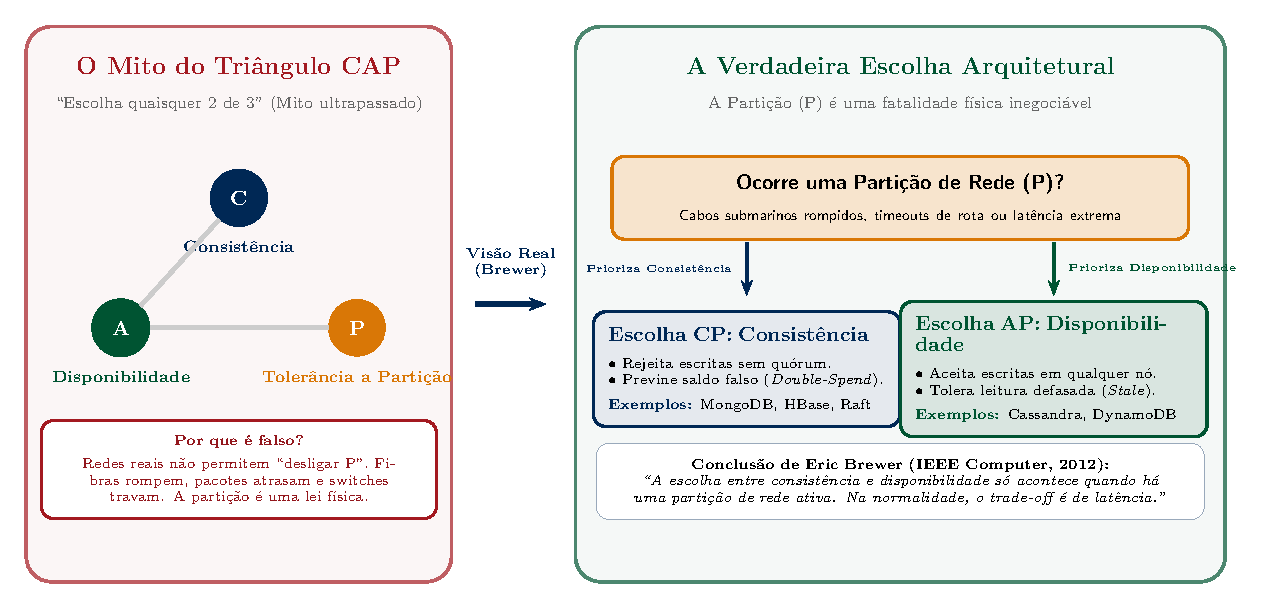
\includegraphics[width=13.6cm,height=4.8cm,keepaspectratio]{figuras/fig_cap_realidade.pdf}%
  }\par
  \vspace{0.15cm}
  \centering
  {\footnotesize \textbf{Regra de Ouro:} \textcolor{ScoutBlue}{Em sistemas distribuídos, a partição é inevitável. Sua única escolha é como agir durante a falha: CP ou AP.}}
\end{frame}

% ------------------------------------------------------------------------------
\twocolframe[title={A Regra de Quórum em Clusters de $N$ Nós},leftcol=7cm,rightcol=7cm]{%
  \alert{A Matemática da Maioria Absoluta}\par
  \itemseps[topsepi=2mm,itemsepi=3mm,labelsep=2mm,leftmargini=4mm]
  \begin{itemize}
    \item Para evitar que duas partes isoladas do cluster gravem dados conflitantes (\textit{Split-Brain}), usa-se o conceito de \textbf{Quórum}:
    \item $$\text{Quórum Mínimo} = \left\lfloor \frac{N}{2} \right\rfloor + 1$$
    \item Onde $N$ é o número total de nós votantes do cluster.
    \item Para $N = 3$ nós: Quórum = $1 + 1 = \mathbf{2 \text{ nós}}$.
    \item Para $N = 5$ nós: Quórum = $2 + 1 = \mathbf{3 \text{ nós}}$.
  \end{itemize}
}{%
  \alert{Por que o Número de Nós deve ser Ímpar?}\par
  \itemseps[topsepi=2mm,itemsepi=3mm,labelsep=2mm,leftmargini=4mm]
  \begin{itemize}
    \item Se tivermos $N = 4$ nós e a rede dividir ao meio (2 e 2), \textbf{nenhum lado tem maioria}! O cluster inteiro para.
    \item Com nós ímpares ($3, 5, 7$), qualquer divisão binária garante que \textbf{apenas um lado} terá a maioria estrita.
    \item O lado maioritário continua operando com segurança. O lado minoritário entra em modo de proteção.
  \end{itemize}
}

% ------------------------------------------------------------------------------
\begin{frame}{Anatomia do Quórum e Partição de Rede (Split-Brain)}
  \vspace{-0.3cm}
  \makebox[\linewidth][c]{%
    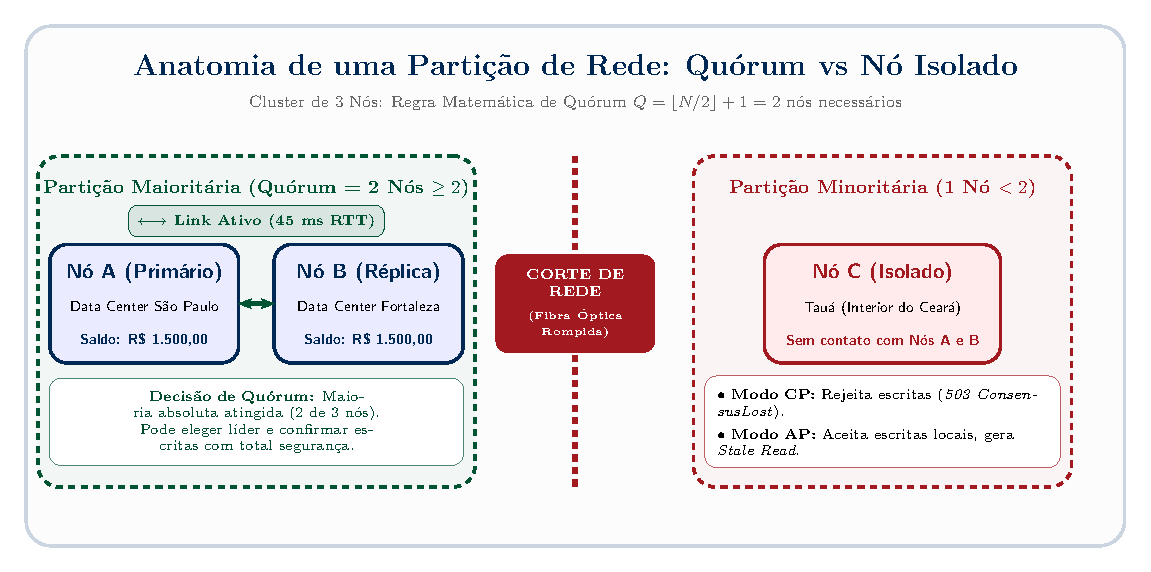
\includegraphics[width=13.6cm,height=4.8cm,keepaspectratio]{figuras/fig_cluster_split_brain.pdf}%
  }\par
  \vspace{0.15cm}
  \centering
  {\footnotesize \textbf{Comportamento:} \textcolor{ScoutBlue}{O lado maioritário (A e B) mantém o quórum de escrita. O nó isolado C deve rejeitar escritas em CP ou aceitar divergência em AP.}}
\end{frame}

% ------------------------------------------------------------------------------
\twocolframe[title={Classificação CAP dos Principais Bancos de Dados},leftcol=7cm,rightcol=7cm]{%
  \alert{Bancos do Tipo CP (Consistência Estrita)}\par
  \itemseps[topsepi=2mm,itemsepi=3mm,labelsep=2mm,leftmargini=4mm]
  \begin{itemize}
    \item \textbf{MongoDB (padrão):} Usa conjuntos de réplicas (\textit{Replica Sets}). Se o primário for isolado da maioria, ele é destituído e recusa escritas.
    \item \textbf{Apache HBase / Bigtable:} Foco absoluto em consistência via ZooKeeper/Raft.
    \item \textbf{Redis (modo Cluster com Quórum):} Rejeita escritas em partições sem mestre válido.
  \end{itemize}
}{%
  \alert{Bancos do Tipo AP (Alta Disponibilidade)}\par
  \itemseps[topsepi=2mm,itemsepi=3mm,labelsep=2mm,leftmargini=4mm]
  \begin{itemize}
    \item \textbf{Apache Cassandra:} Arquitetura \textit{masterless} (todos os nós são iguais). Permite escrita em qualquer nó disponível.
    \item \textbf{Amazon DynamoDB:} Criado especificamente para nunca recusar o carrinho de compras.
    \item \textbf{CouchDB:} Projetado para funcionar offline e sincronizar via HTTP quando a conexão voltar.
  \end{itemize}
}
